\documentclass[10pt]{article}

% amsmath package, useful for mathematical formulas
\usepackage{amsmath}
% amssymb package, useful for mathematical symbols
\usepackage{amssymb}

% graphicx package, useful for including eps and pdf graphics
% include graphics with the command \includegraphics
\usepackage{graphicx}

% cite package, to clean up citations in the main text. Do not remove.
\usepackage{cite}

\usepackage{color} 

% Use doublespacing - comment out for single spacing
\usepackage{setspace} 
\doublespacing

% Text layout
\topmargin 0.0cm
\oddsidemargin 0.5cm
\evensidemargin 0.5cm
\textwidth 16cm 
\textheight 21cm

% Bold the 'Figure #' in the caption and separate it with a period
% Captions will be left justified
\usepackage[labelfont=bf,labelsep=period,justification=raggedright]{caption}

% Use the PLoS provided bibtex style
\bibliographystyle{plos2009}

% Remove brackets from numbering in List of References
\makeatletter
\renewcommand{\@biblabel}[1]{\quad#1.}
\makeatother


% Leave date blank
\date{}

\pagestyle{myheadings}
%% ** EDIT HERE **

\usepackage{multirow}

%% ** EDIT HERE **
%% PLEASE INCLUDE ALL MACROS BELOW

% figure files reside in the figures/ directory
\graphicspath{
{figures/}
}


\usepackage{color}
\usepackage[usenames,dvipsnames]{xcolor}
\usepackage{ulem}

\definecolor{dkred}{rgb}{0.75,0,0}
\definecolor{dkgreen}{rgb}{0,0.5,0}
\definecolor{dkblue}{rgb}{0,0,0.75}
\definecolor{dkpurple}{rgb}{.375,0,.375}
\definecolor{gray}{rgb}{0.5,0.5,0.5}

\newcommand{\removed}[1]{{\color{dkred}\sout{#1}}}
\newcommand{\drew}[1]{{\color{dkgreen}#1}}
\newcommand{\fred}[1]{{\color{dkblue}#1}}
\newcommand{\steph}[1]{{\color{dkpurple}#1}}

%% END MACROS SECTION

\begin{document}

% Title must be 150 characters or less
\begin{flushleft}
{\Large
\textbf{Spatially explicit model of the lymphocyte diaspora in influenza-infected lung reveals thresholds on chemokine directed migration (SUPPLEMENT)}
}
% Insert Author names, affiliations and corresponding author email.
\\
Drew Levin$^{1,\ast}$, 
Stephanie Forrest$^{1}$, 
Soumya Banerjee$^{1}$,
Candice Clay$^{2}$, 
Melanie Moses$^{1}$, 
Frederick Koster$^{1,2}$
\\
\bf{1} Department of Computer Science, University of New Mexico, Albuquerque, NM, USA
\\
\bf{2} Lovelace Respiratory Research Institute, Albuquerque, NM, USA
\\
$\ast$ E-mail: Corresponding drew@cs.unm.edu
\end{flushleft}


% You may title this section "Methods" or "Models". 
% "Models" is not a valid title for PLoS ONE authors. However, PLoS ONE
% authors may use "Analysis" 
\section{Models}

\subsection{CyCells implementation details}

The CyCells modeling environment splits its populations into two types: cells and molecules.  Cells are considered to be unique agents and are modeled individually.  Conversely, molecules are represented as compartmentalized concentrations.  These compartments are arranged as a grid that covers the environment.  Each square in the grid contains a unique concentration of the given molecule.  Each type of  molecule is represented in a unique grid.

Molecular behavior is limited to diffusion and decay.  At each time step, CyCells decreases the concentration of each square in the grid according to the decay rate specified for the given molecule.  CyCells then diffuses the molecules by applying a discrete diffusion equation to each grid square, taking into account the specified diffusion constant and the concentrations in neighboring squares.

New molecules can be secreted by cell objects, such as an infected cell secreting new virus.  In this scenario CyCells calculates the amount of virus secreted per time step, based upon the cell's defined production rate, and then adds this quantity to the grid square that overlaps the secreting cell.  If a cell ingests a molecule, it will subtract the appropriate concentration from the grid square it overlaps.  If the concentration at that square is not enough to represent a full molecule, concentration will be removed from neighboring squares in an ever expanding diamond until the total concentration is equal to a single molecule.

Cells will measure the local concentration at their position by calculating a linearly interpolated combination of the concentrations in the grid squares surrounding the cell in instances where cell behavior depends on the local molecular concentration.


\subsection{Model implementation details}

An overview of the model implementation is shown in Fig. 2.  The model is initialized with one virus-secreting cell placed in the middle of a 2-dimensional sheet of hexagonally-tiled epithelial cells (288,212 total cells).  The sheet measures 5$mm$ per side, which is large enough to contain the infection (Fig. 5).  The molecular grid (Text S1 1.3) is initialized with a resolution of 20$\mu m$.  Each time step of the model represents 6 seconds.

Healthy cells transition to virus-incubating based on a probability that scales linearly with the local virus concentration.   When a cell `becomes infected' it removes the amount of viral concentration equal to a single virion. 

Virus-incubating cells idle for 10 hours (with standard deviation $\sigma=1$ hour) and then transition to virus-secreting cells.  Virus-incubating cells also begin to secrete chemokine after 8 hours (except for aH5N1 which only secretes RANTES after a 16 hour delay).  

Virus-secreting cells secrete both virus and chemokine (the RANTES portion of the chemokine production is added in 16 hours after the initial infection) and die after 1,000 minutes of production (16.7 hours).  Virus-secreting cells will also probabilistically transition to apoptizing cells in the presence of T cells (defined by the existence of a T cell within 2$\mu m$).  The number of T cells in the vicinity of the virus-secreting cell has no effect on the rate that apoptosis is induced in the model.

Apoptizing cells secrete virus and chemokine for one hour and then die.

T cells are added to the model at a constant rate of 1,257 per hour (Text S1 1.1).  Because the model environment is only a small portion of the entire lung (0.25\%), most of the T cells miss the model window and are not visually represented.  The T cells that miss recirculate and enter the lung at a new random location after a delay of six seconds.

The cells that enter the model window are placed at a random position and immediately check the local chemokine concentration.  If the concentration is above the sensitivity threshold, the T cells immediately transition to the chemotaxing state.  If not, the T cells recirculate and reenter the lung in a new location after a six second delay.  Recirculating T cells have a probabilistic decay rate that corresponds to a 3 day lifespan.  Recirculating T cells are not visually represented.  

Chemotaxing T cells move directly up the chemokine gradient until they find a local concentration maximum.  T cells probabilistically decay at a rate corresponding to a 2 hour lifespan.  Chemotaxing T cells have no effect other than inducing apoptosis in virus-secreting cells by proximity.


\subsection{Modeling Decisions}

\subsubsection{Two dimensional lung}

We model the lung as a two-dimensional system for several reasons.  Unlike the lymph node where dendritic cells and T cells navigate a three-dimensional volume, lung infection dynamics are confined to a thin tissue between capillary endothelial cells and alveolar epithelial cells.  Although these alveoli are segregated by the lung's acinar structure on a small scale, we do not represent this in the model because the spreading of influenza eventually ignores the boundaries between acinii.  Therefore our model does not incorporate this small-scale level of segregation.

\subsubsection{Uniform blood flow}

Our model assumes that blood flows uniformly through the lung vascular network.  It is possible that blood flow is increased in the direction of an infected region of the lung by local inflammation.  Thus our model may underestimate the recruitment efficiency of local inflammation and hyperemia.  If this is indeed the case, our model underestimates the effect of the immune response.

%\subsubsection{T cell velocity}
%\fred{T cell velocity in the lung is extremely difficult to measure.} \removed{Little is known of T cell chemotaxis speed in the lung.}  We give chemotaxing T cells a velocity of $3\mu m/s$ and T cells that are performing a random walk a velocity of $30\mu m/s$.  \removed{These values are faster that speeds found in other organs, such as the lymph node.  This is reasonable because T cells in the lung travel on top of a packed surface without needing to navigate through blood flow.  Furthermore, T cell speed has little effect on the model behavior as detailed below (S2.3).}  \fred{These rapid values estimate velocity of capillary blood flow in the extensive network of capillaries beyond the 14th bifurcation of the lung arterial system.  T cell velocity would be expected to be slower within interstitial tissue, but this was not modeled in most simulations.  In runs where velocity was varied over 5 orders of magnitude, including slow velocities measured in lymph node and skin by other authors, T cell velocity had little effect on model behavior and infection control as shown below (S2.3).}
%

%See Table~\ref{table:assumptions}.


% Results and Discussion can be combined.
\section{Results}

\subsection{Estimating chemokine production rates}

We estimate chemokine production rates, `r', by adapting the delay differential equation model of influenza infection described in \cite{Mitchell2011} Eq. 1 by adding one new equation ($\dot{C}=r I_{1 \tau_3}-dC$) to model chemokine production.  Initial population sizes and parameter values are taken from the previous study.
{\footnotesize
\begin{equation}
\begin{aligned}
\dot{T} &= - \beta T V \\
\dot{I_1} &= \beta T V - \beta T_{\tau_1}V_{\tau_1} \\
\dot{I_2} &= \beta T_{\tau_1}V_{\tau_1} - \delta I_2 \\
\dot{V} &= \frac{p}{1+eF} I_2  - \beta T V  \\
\dot{F} &=  I_{1 \tau_2} \\
\dot{C} &= r I_{1 \tau_3} - d C \\
\end{aligned}
\label{eq:dde}
\end{equation}
\vspace{.05in}
}

$\tau$ subscript variables denote delay terms, signifying the value is the population quantity in existence at time $t - \tau$.  Table S1 summarizes population and parameter values and descriptions.  Strain-specific values for $r$ were found by fitting the equations to experimental data (see Results and Table 1).

%\subsection*{Chemokine Secretion}

%To provide estimates of chemokine concentrations and secretion rates present in lung tissue, chemokine levels were measured at 4-6h intervals during the first 48 h of infection in wells containing approximately one million human bronchial epithelial cells (Fig.~\ref{fig:data}).  The dynamic viral loads at these intervals in these cultures infected with seasonal H1N1 virus, pandemic H1N1 virus, and avian H5N1 virus have been reported previously \cite{Mitchell2011}.  IP-10 concentration increases were observed by 8h post-infection (p.i.), and RANTES by 16h p.i..  

%To estimate per-cell chemokine production rates, we extended the delay differential equation (DDE) model of Ref. \cite{Mitchell2011} to include chemokine production from infected cells (Eq.~S1).  Model fits (Table \ref{tab:strains}) were computed for three strains using Matlab's \texttt{nlinfit} function (Levenberg-Marquardt algorithm).  The resulting chemokine production values were used in the CyCells ABM by combining IP-10 and RANTES into one aggregate rate but also reported separately (Fig.~S2).  Best-fit expression rates were similar for all strains except for significantly higher RANTES production in aH5N1.  There was no positive correlation between viral production and induced chemokine production across the three strains.


\subsection{T cell production rate}

We calculate the rate of production ($\sigma$) of CD8 T cells using a differential equation model from \cite{Miao2010}.  The equations model T cell production and subsequent search over an area of infected lung tissue.

{\footnotesize
\begin{equation*}
\label{EqS1}
\begin{aligned}
\dot{N_{c}} &= \sigma - \frac{r'^{2} \cdot N_{c}}{R^{2} \cdot t_{rc}} & \pi r'^{2} &= a \sqrt{I} + b \\
\dot{N'_{f}} &= \frac{(r'^{2} - r^{2}) \cdot N_{c}}{R^{2} \cdot t_{rc}} - \frac{v_{tcell}}{(r' - r) / 2} \hspace*{2cm}  & \pi r^{2} &= \pi r_{cell}^{2} \cdot I \\
\dot{N_{f}} &= \frac{r^{2} \cdot N_{c}}{R^{2} \cdot t_{rc}} + \frac{v_{tcell}}{(r' - r) / 2} \\
\dot{T} &= \rho T -\beta TV \\
\dot{I} &= \beta TV - \delta I - k_{e} N_{f} I \\
\dot{V} &= pI - \beta TV - \gamma (t) V \\
\gamma (t) &= \left\{ \begin{array}{rcl}
	1/\mbox{day} & \mbox{,}  & t < 5  \\
	3/\mbox{day} & \mbox{,} & t \geq 5  
	\end{array}\right. \\
\end{aligned}
\tag{S1}
\end{equation*}
}
\vspace{0.5in}


$N_{c}$ is the number of circulating activated antigen-specific CD8 T cells, $N'_{f}$ is the number of circulating T cells that have found and exit into a region of lung tissue expressing chemokines, $N_{f}$ is the number of circulating T cells that have found an infected region. $T$ is the number of uninfected \textit{target} cells, $I$ is the number of productively infected cells, and $V$ is the viral titer in serum. The infected region is assumed to be of radius $r$ and is within a region expressing chemokines of radius $r'$ ($r  < r'$). The lung is modeled as a circular region with radius $R$. The area of the infected region is equal to the area of an infected cell (of radius $r_{cell}$) multiplied by the number of infected cells. See Fig. 1 for more details about the model.  The area of the region expressing chemokine was found to be related non-linearly to the number of infected cells ($\pi r'^{2} = a \sqrt{I} + b$) where $a$ and $b$ are constants that depend on the viral strain.  $a$ and $b$ were fit using 12 experimental runs of a spatial model implemented in CyCells.

Circulating CD8 T cells ($N_{c}$) are assumed to be released from lymph nodes at a constant rate $\sigma$ and circulate to the $N'_{f}$ population over a time defined by $t_{rc}$. We assume these circulating cells transition into $N'_{f}$ and $N_{f}$ at rates proportional to the areas of the chemokine expressing and infected regions relative to the whole lung area. 

The average time an exiting CD8 T cell takes to migrate to the infected region is equal to the difference in the radii between the two regions ($r' - r$) times the T cell speed, $v_{tcell}$.  Circulating cells that are in the chemokine expressing region ($N'_{f}$) move into the infected region after performing chemotaxis for that time. Target cells ($T$) become infected by virus at rate $\beta TV$, where $\beta$ is the rate constant characterizing infection. Infected cells ($I$) die at rate $\delta$ in addition to being lysed by T cells ($N_{f}$) at a rate $k_{e}$. Finally the viral titers ($V$) increase due to production of virus at rate $p$ by infected cells. Virus is also cleared due to uptake by infected cells (at a rate $- \beta TV$) and due to antibody (at a rate $\gamma (t)$ that changes after 5 days post infection). The initial viral titer was initialized to 10,000 PFUs and the initial number of target cells was one million. The initial number of infected cells is assumed to be zero. Parameter values are listed in Table S1 in Text S1.  This ODE was fit to data taken from \cite{Miao2010} using Matlab's \texttt{nlinfit} function in order to obtain a value for $\sigma$.  The final value was found to be 1,257 per hour.

\subsection{T cell sensitivity to chemokine}

The model simulates a chemokine gradient surrounding the infected focus (Fig. 5), based on the calculated per-infected cell secretion rate (Table 3) and known chemical parameters for a 10 kDa protein (Table 2).  T cell sensitivity depends on receptor density \cite{Desmetz2006} and this was assumed to be constant.

Because this parameter is unknown, we simulated T cell sensitivity levels ranging over 10 orders of magnitude.  Concentration-dependent behavior of cells responding to chemokine was the same over a wide range of concentrations from 0.01 pg/mL to 100 ng/mL (model variance is discussed in Text S1 2.1.).  Decreased recruitment was predicted only by supra-natural concentration sensitivity levels at and above 1 $\mu$g/mL.  We then set the sensitivity to 100 $ng/mL$ for all future runs (10 $nM$ concentration assuming a chemokine molecular weight of 10 $kDa$) \cite{Gao2003}.  

% Because more than one T cell at each infected epithelial cell would not increasing effective target cell death, there may be a threshold of immigrant T cells above which no additional control of viral replication is possible.

\subsection{Chemokine combinations}

Because aH5N1 has been shown to suppress the production of interferon \cite{Mitchell2011}, we hypothesize that it renders IP-10 ineffectual.  We hypothesize that this leads to the elevated RANTES secretion rates measured in aH5N1 compared to the other two strains (Table 3).  Because of this behavior IP-10 was not included in the aH5N1 model runs. 

T cell sensitivity depends on receptor density \cite{Desmetz2006} and this was assumed to be constant.  Thus, the chemokines in combination work additively in our model. 

Four models runs (both, IP-10, RANTES, and none) were performed for sH1N1 and pH1N1 strains and two runs (RANTES and none) for  aH5N1.  The runs show how the presence and/or absence of specific chemokines affect the simulated immune response (Fig.~S\ref{fig:chemokine}).  The lack of both chemokines leads to runaway infections in all three strains.  The presence of only RANTES is enough to contain the aH5N1 infection, but is weaker than IP-10 in both H1N1 strains.  In sH1N1 and pH1N1 simulations, IP-10 alone proves to be as effective as the combination of IP-10 and RANTES.  This suggests that RANTES does not play a significant role in infections that stimulate an IP-10 response due to the higher production rates of IP-10.  


\subsection{General sensitivity analysis}

Model parameters were chosen from literature when available and estimated within plausible ranges otherwise (Table~\ref{tab:parameters}).  Due to the difficulty of estimating critical, unmeasurable values, we performed a sensitivity analysis for 16 parameters in order to test whether variation over an order of magnitude or more altered the infection outcome.  Individual parameters were varied over ranges of plausible (and sometimes even implausible) values while the rest of the parameter set was held constant.  Each parameter was varied over all three influenza strains, creating three sets of sensitivity plots (Figures~\ref{fig:asensitivity}-\ref{fig:psensitivity}).

We then categorize the model parameters into one of three qualitative groups: parameters that do not affect the model's qualitative behavior, parameters that affect the model's peak infection size but do not affect final clearance, and those parameters that affect the final clearance of the infection.  When evaluating the results, we consider model runs that asymptotically converge to be qualitatively stable and model runs that do not converge to be qualitatively divergent.

\subsubsection{Stable Parameters}

The parameters in the first grouping did not affect the outcome of the infection unless they were adjusted to values outside the realm of possibility.  Specifically, each parameter in this group seems to lie within a range that does not significantly affect the asymptotic behavior of the model.  Of interest, this group can be mostly split into two types of parameters: those governing chemokine behavior (chemokine decay, chemokine diffusion, and chemokine secretion) and those governing T cell behavior (T cell circulation time, T cell kill rate, T cell velocity, and the two T cell decay rates).  Only the apoptosis time parameter does not fit into one of these two groups, and its inclusion as a stable parameter may be suspect due to the limited range of the values tested.  The importance of the apoptosis time parameter is discussed in more detail in the main results section: Temporal effects.  

The stability of these parameters makes sense in the context of our model.  Chemokine exists in our model to provide a chemical gradient that T cells may follow to the focus of infection.  The total quantity of the chemokine in the lung does not have a strong effect on the location and size of the gradient.  Thus, the model will be stable for any values of chemokine secretion, diffusion, and decay that provide a gradient that T cells may follow.

Similarly, T cells affect the model by clearing cells expressing virus.  As discussed in the main paper, the chemokine gradient creates areas of maximal concentration that attract all the T cells inside its basin of attraction.  Thus, most T cells are attracted to the same areas of the infection and overlap considerably.  Increasing T cell numbers and efficiency will not help clear the infection beyond a certain point.

While we have claimed that these parameters are qualitatively stable within a certain range, many of the parameters were set to values that did lead to a divergent model behavior.  We have deemed these deviations acceptable on an individual basis as described below.

Apoptosis time diverges slightly in the sH1N1 strain.  As stated earlier, its inclusion in this group is already suspect and its effects are described in more detail in the results section of the main paper.

Varying the chemokine decay rate results in stable model behavior for values one order of magnitude larger and smaller than the default.  A value two orders of magnitude smaller results in divergent behavior for both the aH5N1 strain and the sH1N1 strain and a value two orders of magnitude larger results in divergent behavior for only the sH1N1 strain.  This maximum decay rate used for all three strains corresponds to an implausible 18 second half-life.  The minimal value corresponds to a similarly implausible 50 hour half-life.  The fact that an extremely low decay rate can hinder clearance is interesting.  In this case, lack of decay allows the chemokine to diffuse homogeneously across the entire infection, removing the concentration gradient required by T cells to find the active areas of the infection.  This confirms that the quantity of chemokine is immaterial so long as there is enough for T cells to be able to detect it.  Rather, the presence of chemokine is useful only if its presence results in a chemical gradient surrounding the infection.

The chemokine diffusion rate only diverges in the aH5N1 strain for the highest value.  If anything, our estimate for the diffusion rate is already large as it is optimistically based off of the Stokes-Einstein equation using viscosity of water.  Thus the diffusion rate we used based on Stokes-Einstein and water viscosity was likely within a physiologic range.

Chemokine secretion values differ between strains.  It is important to node that aH5N1 and sH1N1 show a threshold at the same concentration: near 1e-6 $pg/s\cdot cell$.  While this may seem contradictory, it is actually an artifact of our artificially selected chemokine detection threshold, detailed in section S2.1 and Figure~\ref{fig:sensitivity}.  Because we initially picked a sensitivity threshold near the edge of the stable range of possible values, decreasing the total concentration of chemokine inadvertently crosses that arbitrary threshold and does not necessarily suggest an actual region of divergence.

T cell circulation times were tested over a very large range and only diverge at the very edge of that range.  Because vascular and lymph circulation times are unknown, parameter values of 1 minute and 3 minutes in mice may be plausible and warrant further study.

The T cell kill rate only diverges on the lower end in sH1N1.  The extreme value corresponds to a T cell needing 100 minutes to induce the apoptosis of a single infected cell and is not biologically reasonable.  The intermediate value corresponds to a time of 33.3 minutes and is also unlikely.

T cell movement in tissue has been observed \cite{Egen2011}.  Thus, we consider the extreme values biologically implausible.

T cell decay parameters allow the model to diverge only in the most extreme cases.  Neither of these values are reasonable and the parameters show stable behavior otherwise.

\subsubsection{Difference in Peak Only}

Two parameters, viral incubation time and viral expression time, do seem to affect the model's behavior up until the introduction of the T cell response, followed by convergence of infected cell numbers back to the same levels.  This effect occurs because the T cells short circuit the lifespan of infected cells.  Once T cells arrive, virus secreting cells no longer survive for their full lifespan.  Rather, the secretion time becomes limited by the apoptosis time parameter.  Because these terms refer to how and when infected cells release the virus particles, neither one directly affects the kinetics of the virus itself and thus the infection's behavior is still determined by the properties of the virus and the T cell response.

\subsubsection{Unstable Parameters}

This leaves five parameters shown that appear to directly affect the result of the infection: IgM strength, infection sensitivity, T cell secretion rate, viral decay, and viral diffusion.  By comparing the three strains of influenza, we also know that the viral secretion rate affects the result.  Of interest, nearly all of these parameters are directly related to the behavior of the virus.  Only the T cell secretion rate and IgM parameters are not.  

IgM strength is not inserted until day 4 of the simulation, but once it does it directly affects the decay rate of the virus, and does so for the rest of the simulation.  The higher the strength of this parameter, the less virus there is in the system.  Because the true effective strength of IgM is unknown in the context of this model, it is not a target of our investigation. 

Viral decay has the exact same effect as the IgM strength parameter.  Its value directly determines how much virus remains in the system over the course of the infection.

Infection sensitivity describes the ability of the virus to infect healthy cells, yet its strength is directly related to how much virus is present in the area of the healthy cells.  Thus, increasing its value by any factor is equivalent to increasing the amount of virus by the same factor.  Thus, it behaves similarly to the IgM and viral decay parameters.

Shown elsewhere, the viral secretion rate has a strong effect on the outcome of the infection.  Similar to the previously discussed parameters, its value directly affects how much virus there is in the system.  Thus, it's affect is similar to the previous parameters.

Viral diffusion does not change how much virus there is in the system.  Rather, it determines how fast the virus may spread across the alveoli.  While its mechanism is different, its effect may be even stronger than the previous parameters.  By allowing the virus to diffuse faster than the chemokine (an unlikely scenario), the virus spread may outpace the body's ability to generate a chemical gradient.  Thus T cells will constantly be directed to locations behind the front edge rapidly spreading viral cloud and will be unable to 'get ahead' of the spread of the infection.

Finally, the T cell secretion rate does have a consistent response over its different values, but this effect is minimized above a certain rate.  Thus it is reasonable to assume that there is a threshold of T cell secretion, beyond which the dynamics of the infection do not change.  This is consistent with our observations of T cell clumping in areas of high chemokine concentration.  Increasing the number of T cells in the system does not seem to help beyond a certain point because the T cells overlap in space and become redundant.


%\drew{
%\subsection{T cell speed}
%
%\removed{T cell speed over bronchial epithelial cells is unknown.}\fred{T cell velocity within the capillary network and after diapedesis with the lung interstitial tissue is unknown.}  We tested values for T cell speed to measure the effect it had on the general infection dynamics (Fig.~S\ref{fig:speed}).  The results show that the difference in T cell speeds is small, although there does appear to be an discernible effect on the infection during \removed{the early phase of the T cell response} \fred{the initial appearance of activated T cell migration between days 5 and 7 post infection.}.
%}

\section{Discussion}

\subsection{Chemokine directed T cell search}

The \textit{in vivo} quantitative chemokine parameters in the infected lung are difficult to estimate.  Blood levels documented in virulent influenza infections \cite{DeJong2006} may not reflect lung tissue concentrations.  Dynamic chemokine concentrations secreted by bronchial epithelial cells \textit{in vitro} depend on infection intensity and cell maturation state \cite{Mitchell2011, Chan2010, Chan2005, Zeng2011} but may better approximate tissue levels.  Interestingly, the attenuation of the type I interferon response by H5N1 viruses is not associated with attenuation of chemokine secretion in our results and in others \cite{Zeng2007}.  The model did not incorporate the potential contributions from other chemokines such as CXCL8/IL-8 detected in bronchial cell cultures \cite{Matsukura1996, Arndt2002}, nor did the model account for chemokines secreted by immigrant macrophages \cite{Julkunen2000} and amplification of epithelial cell secretion by CD8 T cells \cite{Zhao2000}.

A key determinant in the efficiency of chemokine-directed T cell migration towards virus-secreting epithelial cells is the communication distance, defined by the threshold of sufficient chemokine signal required to induce directed motion of the cell up the chemical gradient \cite{Thelen2008}.  The diameter of this gradient generated by a single cell is a function of production rate, decay rate, protein diffusion and the sensitivity threshold.  For the threshold of 100 ng/mL and maximal levels of concentration in tissue of 10,000 ng/mL, we calculated the effective communication distance to be approximately 100 microns in our model by simulating a single chemokine producing cell and observing the radius of the resulting chemokine gradient.  This calculation is similar to the distance calculated for generic cytokines secreted by a suspended solitary cell \cite{Francis1997}.  

Future work with spatially explicit modeling should explore the communication distance in more detail, as well as the role of immigrant CD8 T cell proliferation, contribution of resident memory T cells and B cells, and effector cell lifespan. 

% The bibtex filename
\bibliography{references}

\pagebreak

\section*{Figure Legends}

%\begin{figure}[!ht]
%\begin{center}
%%\includegraphics[width=4in]{figure_name.2.eps}
%\end{center}
%\caption{
%{\bf Bold the first sentence.}  Rest of figure 2  caption.  Caption 
%should be left justified, as specified by the options to the caption 
%package.
%}
%\label{Figure_label}
%\end{figure}


\setcounter{figure}{0}
\renewcommand{\thefigure}{S\arabic{figure}}


\begin{figure}[!ht]
\begin{center}
 \includegraphics[width=\textwidth]{Figure_S1}
 \end{center}
\caption{{\bf Varying T cell sensitivity to chemokine.}  H5N1 model results use RANTES  only, and sH1N1 and pH1N1 use both IP-10 and RANTES. Total number of incubating, secreting and apoptotic cells are plotted for each infection.  The sensitivity value specifies the minimum level of chemokine concentration required for T cells to detect it. } 
 \label{fig:sensitivity}
\end{figure}


\begin{figure}[ht!]
\begin{center}
	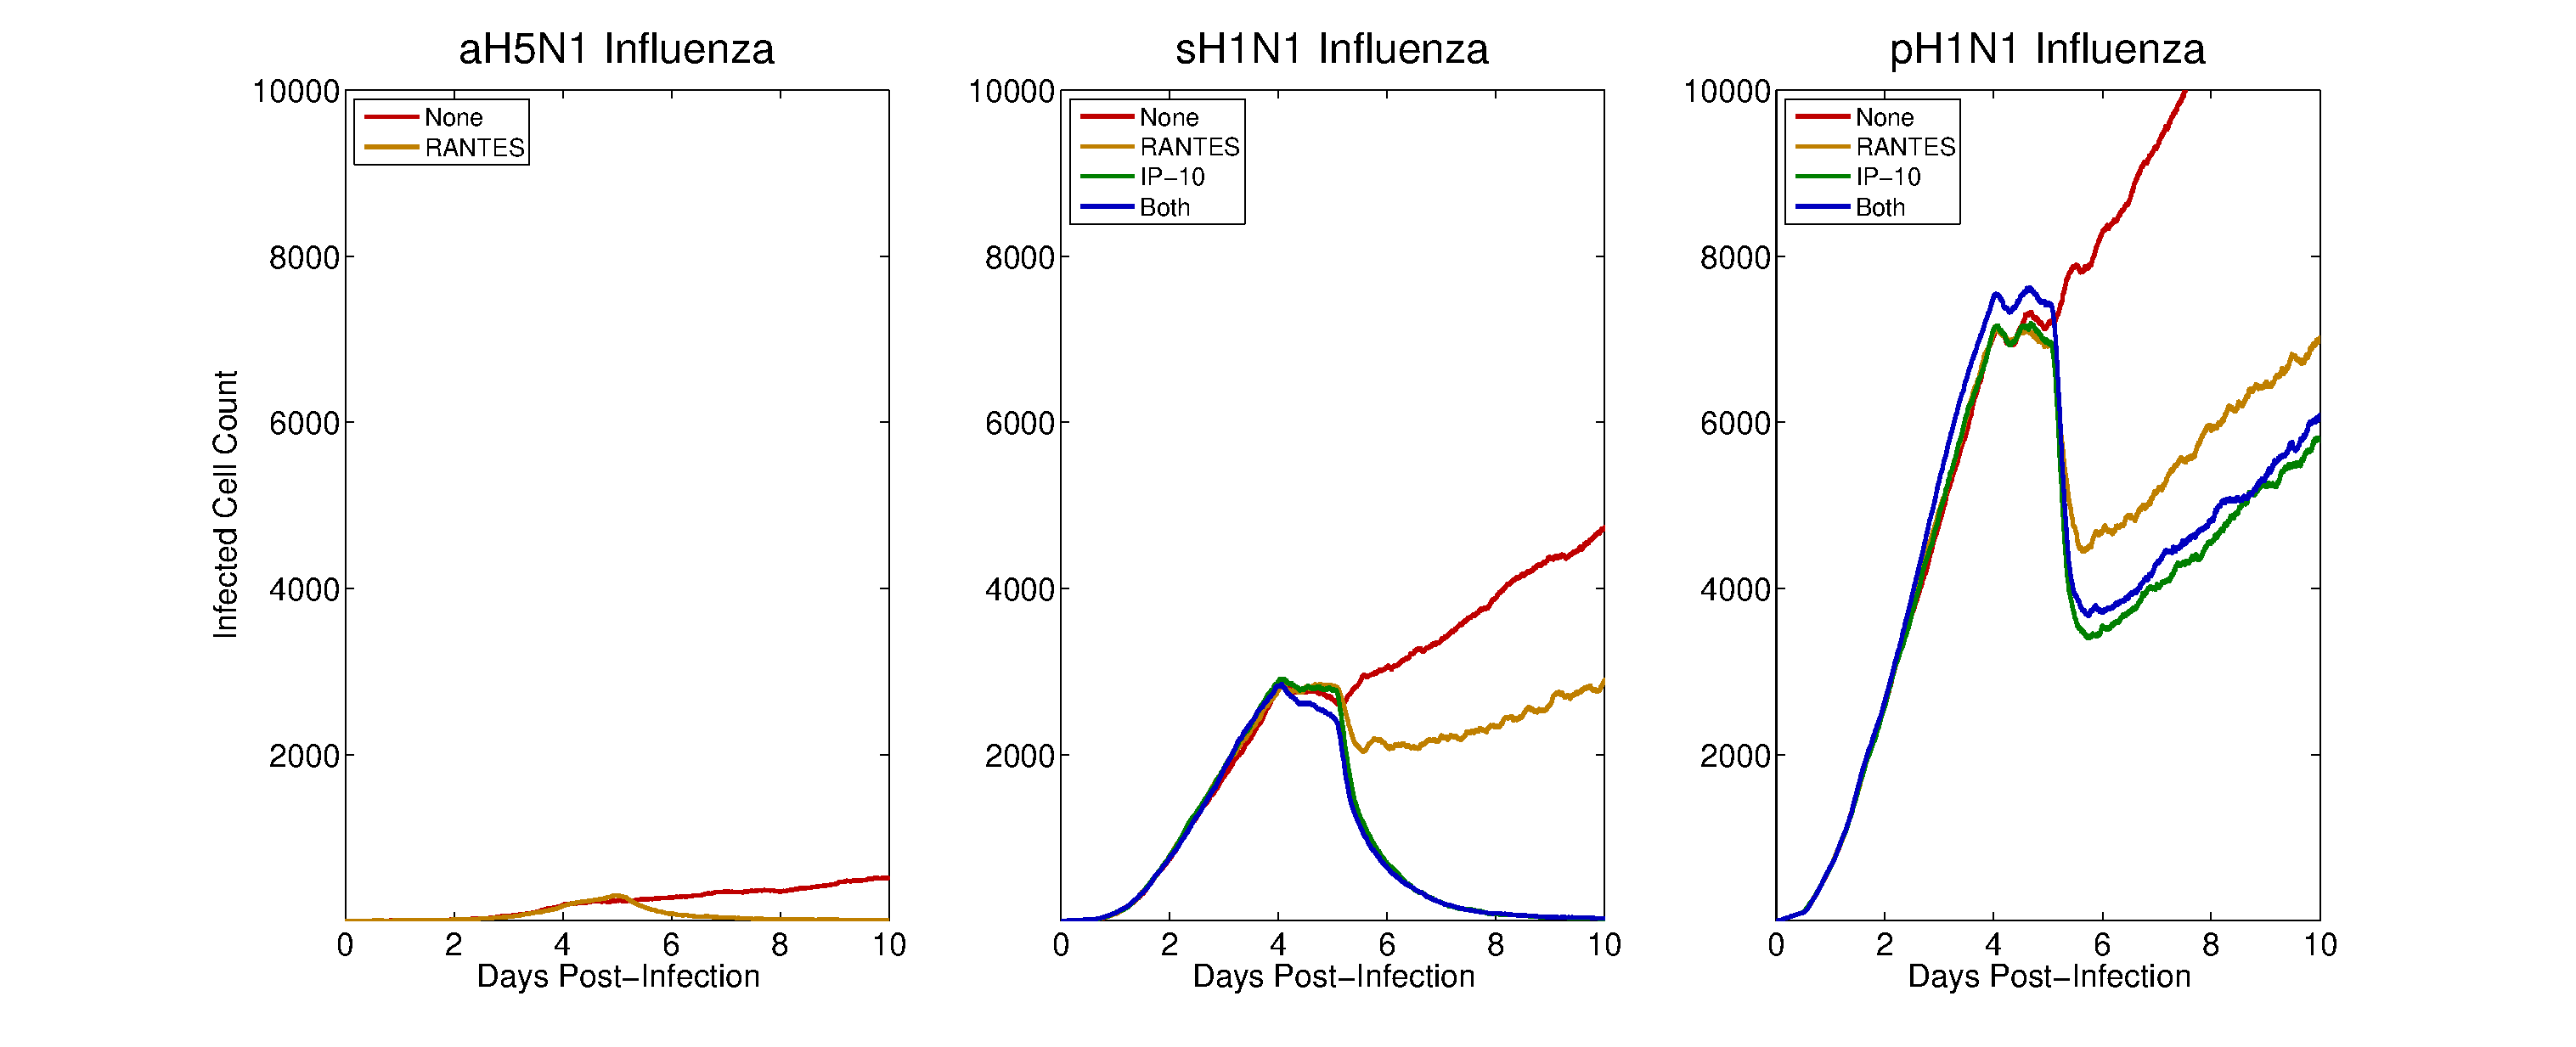
\includegraphics[width=\textwidth]{Figure_S2}
	\caption{\textbf{Effects of different chemokine combinations.}  A) aH5N1 does not stimulate an IP-10 response.  B-C) sH1N1 and pH1N1 show no significant difference between IP-10 alone versus IP-10 and RANTES combined.}
	\label{fig:chemokine}
\end{center}
\end{figure}

%\begin{figure}[ht!]
%\begin{center}
%	\includegraphics[width=\textwidth]{Figure_S3}
%	\caption{\drew{\textbf{Effects of different T cell speeds.}  With the exception of sH1N1, T cell speeds show a small effect during the early phase of the T cell response.  After a time of approximately two days, the infection dynamics converge to a similar rate of growth across all speed values.}}
%	\label{fig:speed}
%\end{center}
%\end{figure}

\setcounter{figure}{0}
\renewcommand{\figurename}{Video}


\begin{figure}[ht!]
\caption{The first of three overlaid videos of a representative seasonal H1N1 infection.  This video spans the 10 day infection and shows the cells as they transition from healthy to infected to dead.  T cells show half way through the simulation.  Healthy cells are gray, virus-incubating cells are yellow, virus-secreting cells are orange, apoptotic cells are red, and T cells are green.} 
 \label{video:cell_view}
\end{figure}

\begin{figure}[ht!]
\caption{The second of three overlaid videos of a representative seasonal H1N1 infection.  This video spans the 10 day infection and shows the virus concentration.  Notice the volatility when T cells arrive halfway through the simulation.  Virus concentration ranges from 1e-13 mols/mL (white) to 1e-27 mols/mL (black).  Refer to Figure 5 for the detailed legend. } 
 \label{video:virus_view}
\end{figure}

\begin{figure}[ht!]
\caption{The third of three overlaid videos of a representative seasonal H1N1 infection.  This video spans the 10 day infection and shows the chemokine concentration.  Notice the volatility when T cells arrive halfway through the simulation.  Chemokine concentration ranges from 1e8 ng/mL (white) to 1e-6 ng/mL (black).  Refer to Figure 5 for the detailed legend. } 
 \label{video:chemokine_view}
\end{figure}

\begin{figure}[ht!]
\caption{A closer look at the 2009 pandemic simulation.  This video shows the infection from day 6 to day 7 with each frame spanning 1 simulated minute.  Healthy cells are gray, virus-incubating cells are yellow, virus-secreting cells are orange, apoptotic cells are red, and T cells are green.  Note the high proportion of virus-secreting cells (orange) early on.  As time passes, secreting cells are gradually contained to the point where they become very sparse.  T cell clumping often prevents the T cells from quick discovery of new secreting cells.}
\end{figure}

\pagebreak

\section*{Tables}

%\begin{table}[!ht]
%\caption{
%\bf{Table title}}
%\begin{tabular}{|c|c|c|}
%table information
%\end{tabular}
%\begin{flushleft}Table caption
%\end{flushleft}
%\label{tab:label}

% \end{table}

\renewcommand{\thetable}{S\arabic{table}}

\begin{table}
\begin{center}
\begin{tabular}{|  l  l  l  |}
  \hline
  Population & Description & Initial Value\\
  \hline
  $T$ & Healthy target epithelial cells & 1,000,000 \\
  $I_1$ & Virus-incubating cells & 0 \\
  $I_2$ & Virus-secreting cells & 0 \\
  $V$ & Free virus particles & 10,000 \\
  $F$ & Interferon quantity & 0 \\
  $C$ & Chemokine quantity (ng/mL) & 0 \\
  \hline
  \hline
  Parameter & Description & Value \\
  \hline
  $\beta$ & Viral infection rates &  \\
    & \hspace{2em} Avian & 5.3e-7 (PFU$\cdot$h)$^{-1}$ \\
    & \hspace{2em} Seasonal & 6.1e-7 (PFU$\cdot$h)$^{-1}$ \\
    & \hspace{2em} Pandemic &  2.7e-6 (PFU$\cdot$h)$^{-1}$\\
  $p$ & Viral production rates & \\
    & \hspace{2em} Avian & 0.20 (PFU/h) \\
    & \hspace{2em} Seasonal & 1.4 (PFU/h) \\
    & \hspace{2em} Pandemic & 18.3 (PFU/h) \\
  $e$ & Interferon strengths & \\
    & \hspace{2em} Avian & 1.0e-8 \\
    & \hspace{2em} Seasonal & 1.6e-6 \\
    & \hspace{2em} Pandemic & 3.4e-3 \\
  $\tau_2$ & Interferon production delays &  \\
    & \hspace{2em} Avian & 21.5 (h) \\
    & \hspace{2em} Seasonal & 23.6 (h) \\
    & \hspace{2em} Pandemic & 21.0 (h) \\
  $\delta$ & Virus-secreting cell decay rate & 0.6 (h$^{-1}$) \\
  $d$ & Chemokine decay rate & 1.386 (h$^{-1}$) \\
  $\tau_1$ & Viral incubation time & 10 (h) \\
  $\tau_3$ & Chemokine production delays & \\
    & \hspace{2em} IP-10 & 8 (h)\\
    & \hspace{2em} RANTES & 16 (h)\\
  \hline
\end{tabular}
\caption{All parameters and populations are taken from \cite{Mitchell2011} except for $C$, $d$, and $\tau_3$.  The value chosen for $d$ corresponds to a 30 minute half-life and values for $\tau_3$ were set from the observed chemokine data (Fig.~\ref{fig:data}).  Interferon ($F$) is an abstracted unitless quantity and thus $e$ is a unitless multiplier.}
\label{tab:dde}
\end{center}
\end{table}


\begin{table}[!ht]
\begin{center}
\begin{tabular}{ | c | c | c | }
  \hline                        
  Paramter & Value & Source \\
  \hline
  T(0) & $1e6$ & \cite{Mitchell2011} \\
  V(0) &  $1e4$ & \cite{Mitchell2011} \\
  $r_{cell}$ &  $5 \mu m$ & \cite{Miao2010} \\
  $t_{rc}$ & $6s$ & \cite{Peters1983} \\
  $k_e$ & $6.4e-5/cell/day$ & \cite{Miao2010} \\
  $\beta$ & $4.8e-7/cell/PFU$ & \cite{Mitchell2011} \\
  $p$ & $0.18 PFU/h$ & \cite{Mitchell2011} \\
  $\delta$ & $16.7 hours$ & \cite{Mitchell2011} \\
  $a$ & $67.7$ & ABM fits \\
  $b$ & $433.5$ & ABM fits \\
  \hline  
\end{tabular}
\caption{Supplemental model parameters.  Most values are chosen to match the equations borrowed from both \cite{Mitchell2011} and \cite{Miao2010}.  Values \textit{a} and \textit{b} were fit to multiple runs of a simplified CyCells ABM.}
\label{table:supplement}
\end{center}
\end{table}

%\begin{table}[!ht]
%\begin{center}
%\begin{tabular}{ | c | c | }
%  \hline                        
%  Assumption & Description \\
%  \hline
%  2D hexagonal layout & The lung can be stretched flat.  T cells travel on the cellular surface. \\
%  Even blood flow to all capillaries & We assume that there is negligible increased blood flow to the infected region. \\
%  Rapid T cell circulation & Activated T cells in circulation do not spend time in new lymph nodes as they circulate. \\
%  T cell speed & T cells move at a rate of XXX in the absence of chemokine and XXXX once it detects chemokine. \\
%  T cell search time & T cells search in the lung for 6 minutes before they recirculate. \\
%  \hline  
%\end{tabular}
%\caption{Supplemental model parameters.  Most values are chosen to match the equations borrowed from both \cite{Mitchell2011} and \cite{Miao2010}.  Values \textit{a} and \textit{b} were fit to multiple runs of a simplified CyCells ABM.}
%\label{table:assumptions}
%\end{center}
%\end{table}

\end{document}
